\documentclass[12pt, oneside]{article}
\usepackage[letterpaper, margin=1in]{geometry}
\usepackage[english]{babel}
\usepackage[utf8]{inputenc}
\usepackage{amsmath}
\usepackage{amsfonts}
\usepackage{amssymb}
\usepackage{tikz}
%\usepackage{tkz-fct}
\usepackage{pgfplots}
\pgfplotsset{width=10cm,compat=1.9}
\usepgfplotslibrary{statistics}
\usepackage{pgfplotstable}
%\usepackage{venndiagram}

\usepackage{fancyhdr}
\pagestyle{fancy}
\fancyhf{}
\rhead{\thepage \\Name: \hspace{1.5in}.\\}
\lhead{BECA / Dr. Huson / 11.2 Algebra 2\\* 7 May 2018 \\*\textbf{Homework: Pretest exponential functions
}}

\renewcommand{\headrulewidth}{0pt}

\begin{document}


%\subsection*{Solve equations}

%Solve for the value of $x$.
\vspace{1cm}

\begin{enumerate}


\item A bank account earns interest at a continuous interest rate of 5\% per year. The initial deposit is \$225.
\begin{enumerate}
    \item Express the balance in the account as a function in the form $P(t)=P_0 \cdot e^{rt}$\\[30pt]
    \item Convert the function to one without a coefficient in the exponent. \\[30pt]
    \item What is the interest rate expressed as a simple, annual rate?\\[30pt]
\end{enumerate}

\item Judith puts \$5000 into an investment account with interest compounded continuously. If the annual interest rate is 3.25\% what is the balance after 30 years?\\[80pt]

\item The function below models the average price of gas in a small town since January 1st.
\[G(t)=-0.0049t^4 + 0.0923t^3 - 0.56t^2 +1.166t+3.23 \text{, where } 0 \leq t \leq 10.\]
If $G(t)$ is the average price of gas in dollars and $t$ represents the number of months since January 1st, the absolute maximum $G(t)$ reaches over the given domain is about what value, to the nearest cent? (graph the function in your calculator and use the Max function)%Alg2 Regents Jan2018

\newpage


\item Write $\sqrt[3]x^8$ as a single term with a rational exponent.\\*[30pt]

\item Write $\sqrt{a^3} \div a^{\frac{1}{2}}$ as an expression with positive, integer exponents.\\*[30pt]

\item If $n=\sqrt{z^5}$ and $m=z$, where $a > 0$, express $\frac{n}{m}$ as 
\begin{enumerate}
    \item a radical with positive, integer exponents\\*[30pt]
    \item an expression with a fractional exponent\\*[30pt]
\end{enumerate}

\item What is the expression $5i^3(-2i+5)$ is equivalent to? Express your answer in the form $a+bi$, where $a, b \in \mathbb{R}$.\\*[30pt]  %Alg2 Regents Jun2017 multiple choice

\item Simplify the expression $(2x - i)^2$, where $i$ is the imaginary unit. Express your answer in the form $a+bi$, where $a, b \in \mathbb{R}$.\\[30pt] %Alg2 Regents Aug2017

\item Algebraically determine the values of $h$ and $k$ to correctly complete the identity stated below.
\[3x^3-7x^2+5x-7=(x-2)(3x^2+hx+3)+k\] %Alg2 Regents Jan 2017

\newpage
\item Graph the function $f(x)=x^3-4x+1$. 
\begin{enumerate}
    \item Write down the $y$-intercept.\\*[10pt]
    \item Mark the $x$-intercepts on the graph as ordered pairs, rounding to the nearest hundredth.\\*[10pt]
    \item Describe the end behavior of the function. (use language like "As $x$ goes to positive infinity, $y$ goes to...")\\*[50pt]
\end{enumerate}

\begin{figure}[!ht]
    \centering
    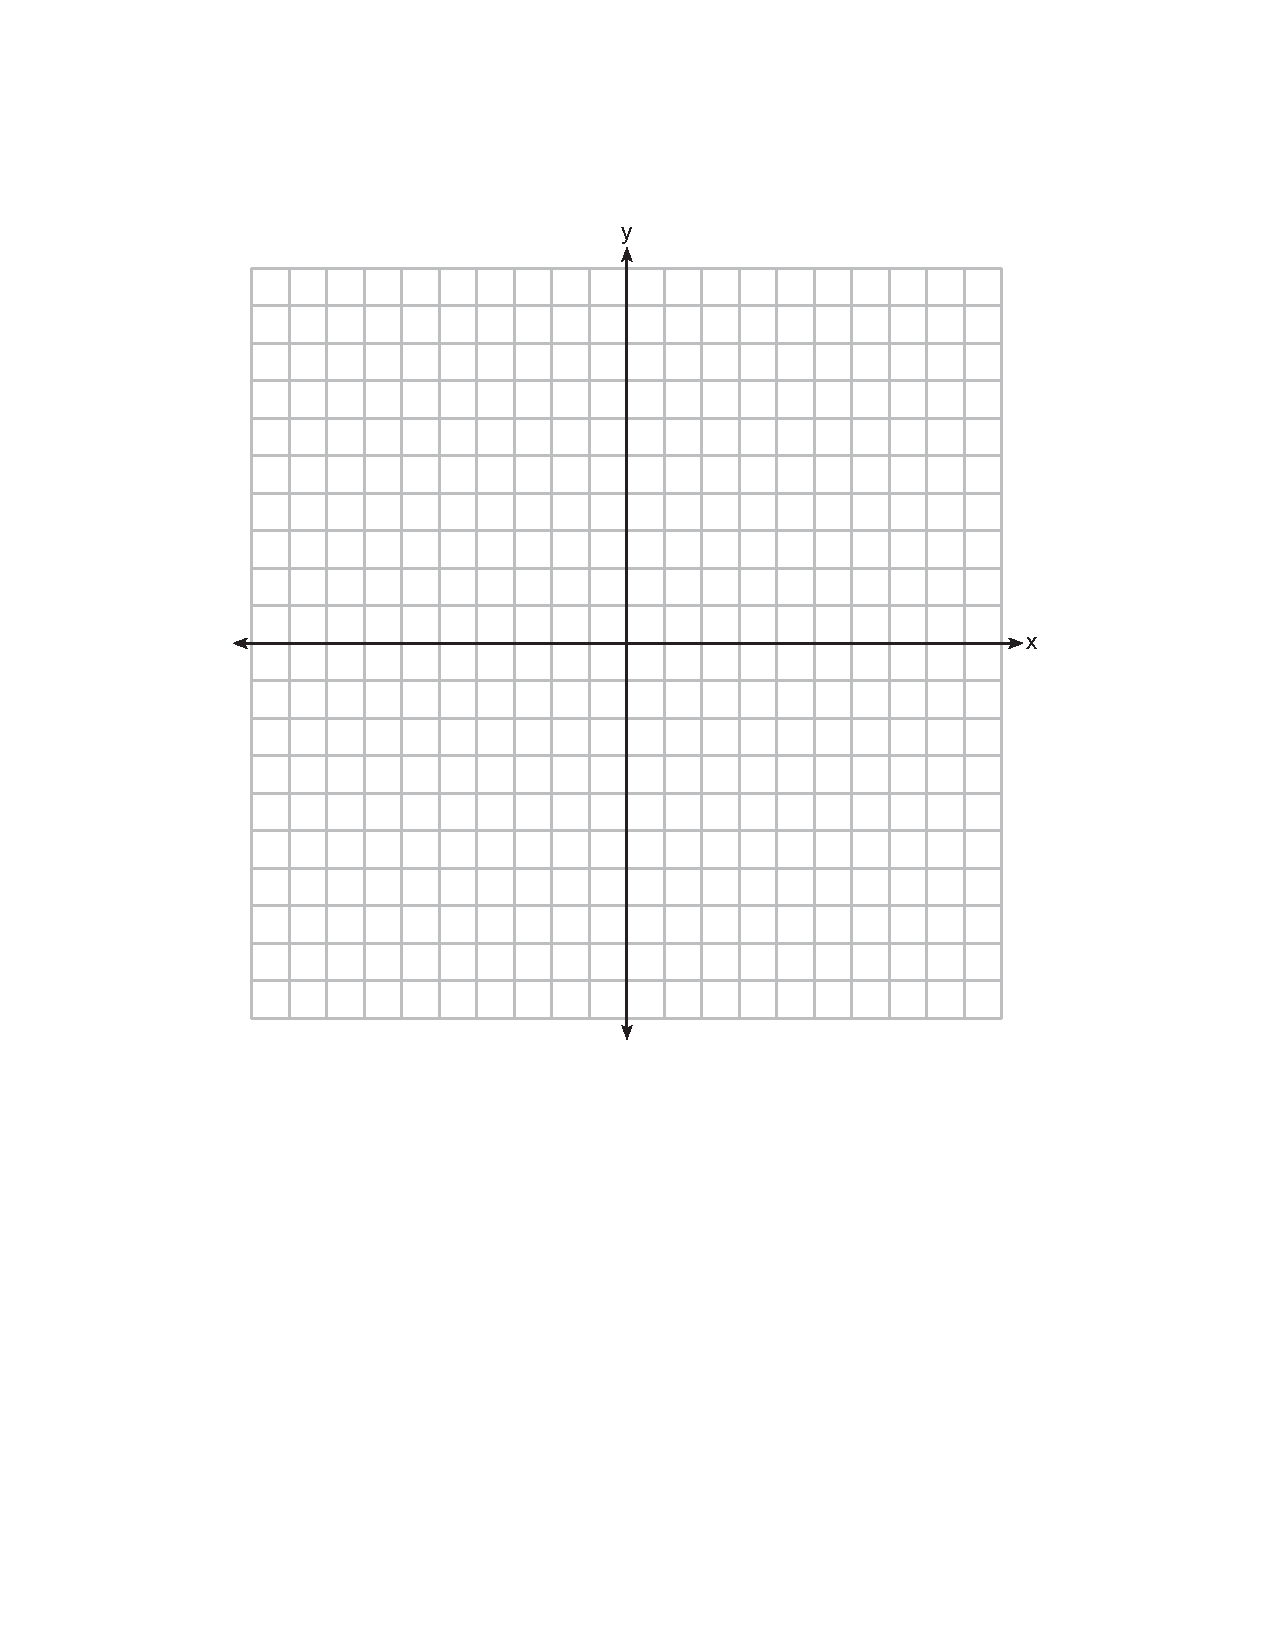
\includegraphics[width=0.75\textwidth]{regents-grid.pdf}
\end{figure}

\newpage
\item The expression $(x + a)(x + b)$ can not be written as
\begin{enumerate}
    \item $a(x + b)+ x(x + b)$
    \item $x^2 + (a + b)x + ab$ 
    \item  $x^2 + abx + ab$  
    \item $x(x + a)+ b(x + a)$
\end{enumerate}

\item What is the quotient when $3x^3+9x^2+8x+5$ is divided by $x+2$?\\*[50pt]

\newpage
\item Judith puts \$1000 into an investment account with interest compounded continuously. What is the approximate annual rate is needed for the account to grow to \$1529.59 after 10 years?

\item The function $p(t)=110e^{0.03922t}$ models the population of a city, in millions, $t$ years after 2010.
\begin{enumerate}
    \item Initially, as of 2010, what is the population in millions.\\[40pt]
    \item What is the rate that the population increases continuously, per year?\\[40pt]
    \item Express the population as a function with the form $p(t)=Ab^{t}$, where $A$ and $b$ are real numbers.\\[40pt]
\end{enumerate}

\item For a given time, $x$, in seconds, an electric current, $y$, can be represented by $y = 2.7^{-.10x}$. 
\begin{enumerate}
    \item Simplify the expression to eliminate the coefficient in the exponent.\\[40pt]
    \item Is the electric current increasing or decreasing? Justify your answer.\\[70pt]
    \item Is the current in the original equation, above, exponential growth or decay? Why?\\[70pt]
\end{enumerate}

\newpage

\item Iridium-192 is an isotope of iridium and has a half-life of 73.83 days. If a laboratory experiment begins with 100 grams of Iridium-192, the number of grams, $A$, of Iridium-192 present after $t$ days would be 
\[A=100 \left( \frac{1}{2} \right)^\frac{t}{73.83}\]

\begin{enumerate}
    \item Simplify the equation to eliminate the fraction in the exponent.\\[30pt]
    \item After one day, how much isotope is present?\\[30pt]
    \item As a percentage, how much does the mass of the isotope change each day?\\[30pt]
\end{enumerate}


\end{enumerate}
\end{document}